%\documentclass[tikz, border=5pt]{standalone}
\begin{document}
	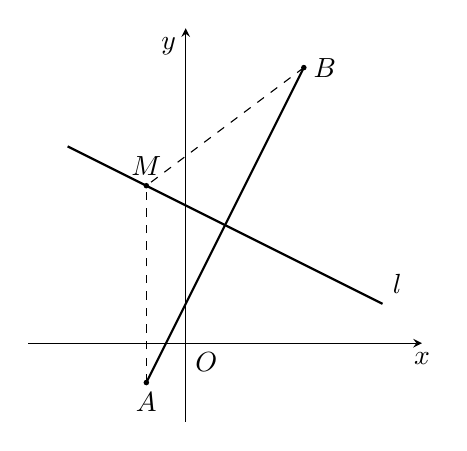
\begin{tikzpicture}[>=stealth, scale=0.5]
		% 绘制坐标轴
		\draw[->] (-4,0) -- (6,0) node[below] {$x$}; % x轴(带箭头和标签)
		\draw[->] (0,-2) -- (0,8) node[below left] {$y$}; % y轴(带箭头和标签)
		\node at (0,0) [below right] {$O$};           % 原点O的标签
		
		% 直线l  x+2y−7=0
		\draw[thick] (-3, 5) -- (5, 1) node[above right] {$l$}; 
		
		% 定义各关键点坐标
		\coordinate (A) at (-1,-1);  % 点P₁
		\coordinate (B) at (3,7); % 点P₂
		\coordinate (M) at (-1,4);  % 点M₁
		
		% 绘制连线
		\draw[thick] (A) -- (B);  % Q到P₁的虚线
		\draw[dashed] (A) -- (M); % P₁到x轴的虚线
		\draw[dashed] (B) -- (M); % P₂到y轴的虚线
		
		% 标记各点的标签
		\fill (A) circle (2pt) node[below] {$A$};  % 绘制点A
		\fill (B) circle (2pt) node[right] {$B$};   % 绘制点B
		\fill (M) circle (2pt) node[above] {$M$};    % 绘制点M
		
	\end{tikzpicture}
\end{document}
